\documentclass[border=8pt, multi, tikz]{standalone} 
\usepackage{import}
\subimport{layers/}{init}
\usetikzlibrary{positioning}
\usetikzlibrary{3d} %for including external image 

\tikzset{
  font={\fontsize{15pt}{15}\selectfont}
}

\def\lineColor{black!90}
\def\inputColor{rgb:yellow,3;green,2;red,1}
\def\ConvColor{rgb:yellow,5;red,5;white,5}
\def\PoolColor{rgb:blue,30;green,10}
\def\FcColor{rgb:blue,5;red,2.5;white,5}
\def\FcReluColor{rgb:blue,5;red,5;white,4}
\def\SoftmaxColor{rgb:magenta,5;black,7}
\def\LossColor{rgb:magenta,5;black,5}

\def\layerSeparation{5}

%\def\inputWidth{28}
%\def\cnnWidth{26}
%\def\filtersCount{8}
%\def\maxPoolWidth{13}
%\def\fcHalfNodes{4}
%\def\outputnodes{9}

\def\inputWidth{6}
\def\cnnWidth{4}
\def\filtersCount{1}
\def\maxPoolWidth{2}
\def\fcHalfNodes{3}
\def\outputnodes{4}

\tikzstyle{neuron}=[circle,draw=black,fill=cyan!65,line width=0.001mm,minimum size=3em,inner sep=0pt]
\tikzstyle{connection}=[line width=0.5mm,every node/.style={sloped,allow upside down},draw=\lineColor,opacity=0.7] 
\tikzstyle{connectionNN}=[->,line width=0.2mm,draw=\lineColor,opacity=0.7]
\tikzstyle{captionlabel}=[text width=5em,text centered]
\tikzstyle{box}=[rectangle,draw=black,fill=\LossColor,opacity=0.5,minimum size=4.5em,inner sep=0pt]
\tikzstyle{annot}=[font=\fontsize{17}{0}\selectfont,text width=7em, text centered]

\newcommand{\inputLayer}{ 
    %\node[canvas is zy plane at x=0] (temp) at (\layerSeparation*0,0,0) {\includegraphics[width=6cm,height=6cm]{mnist_digit.png}};
    \pic[shift={(0,0,0)}] at (0,0,0) {
        Box={ 
            name=input,
            caption=Input,
            xlabel={{1, }},
            zlabel=\inputWidth,
            fill=\inputColor,
            height=28,
            width=1,
            depth=28
            } 
        };
}

\newcommand{\convolutionLayer}{ 
    \pic[shift={(0,0,0)}] at (\layerSeparation*1,0,0) 
    {Box={
        name=conv1,
        caption=Convolution,
        xlabel={{\filtersCount,}},
        %xlabel={{,,,,\filtersCount,,,}},
        zlabel=\cnnWidth,
        fill=\ConvColor,
        height=26,
        width=1,
        %width={1,1,1,1,1,1,1,1},
        depth=26
    }
    };
    \node[below right=7em of conv1-north] {$out_{conv}$};
}

\newcommand{\maxPoolLayer}{ 
\pic[shift={(0,0,0)}] at (\layerSeparation*2,0,0) 
    {Box={
        name=max_pool1,
        caption=Max Pool,
        xlabel={{\filtersCount,}},
        %xlabel={{,,,,\filtersCount,,,}},
        zlabel=\maxPoolWidth,
        fill=\PoolColor,
        height=13,
        width=1,
        %width={1,1,1,1,1,1,1,1},
        depth=13
    }
    };
    \node[below right=3em of max_pool1-north] {$out_{mp}$};
}


\newcommand{\fullyConnectedLayer}{ 
    \foreach \i in {1,...,\fcHalfNodes}
        \node[neuron] (fc-up\i) at (\layerSeparation*3, \i * 1.4) {};
    
    \node (fc-ell) at (\layerSeparation*3, 0) {\vdots};
    \foreach \i in {1,...,\fcHalfNodes}
        \node[neuron] (fc-down\i) at (\layerSeparation*3, \i * -1.4) {};
    
    \node[annot,above right=1em of fc-up\fcHalfNodes.east] {$out_{fc}$};
    \node[below of=fc-down\fcHalfNodes,node distance=4em,captionlabel] {\textcolor{black}{ \bf Fully\\connected layer}}; 
}

\newcommand{\softmaxLayer}{ 
    \foreach \i in {0,...,\outputnodes}
        \node[neuron] (softmax-\i) at (\layerSeparation*4, \i * 1.4 - \outputnodes/2 - 0.5) {$p_{\i}$};
    
    \node[annot,above right=-1.5em of softmax-\outputnodes.east] {$out_{s}$};
    \node[below of=softmax-0,node distance=3em,captionlabel] {\textcolor{black}{ \bf Softmax}}; 
}

\newcommand{\lossLayer}{ 
    \node[box, right of=softmax-3] (L) at (\layerSeparation*5, 0) {L};
    \node[below of=L,node distance=4em,captionlabel] {\textcolor{black}{ \bf Loss}};
}

\begin{document}
\begin{tikzpicture}
    \inputLayer

    \convolutionLayer

    \draw [connection]  (input-east)    -- node {\midarrow} (conv1-west);

    \maxPoolLayer

    \draw [connection]  (conv1-east)    -- node {\midarrow} (max_pool1-west);
    \fullyConnectedLayer

    \draw [connection]  (max_pool1-east)    -- node {\midarrow} (fc-ell);

    \softmaxLayer
    
    % Draw connections from fully connected layer to softmax
    \foreach \i in {0,...,\outputnodes} {
        \foreach \j in {1,...,\fcHalfNodes} {
            \draw[connectionNN] (fc-up\j) edge (softmax-\i);
            \draw[connectionNN] (fc-down\j) edge (softmax-\i); 
        }
    }

    \lossLayer

    \foreach \i in {0,...,\outputnodes} {
        \draw[connectionNN] (softmax-\i) edge (L);
    }
\end{tikzpicture}

\begin{tikzpicture}
    \inputLayer

    \convolutionLayer

    \draw [connection]  (input-east)    -- node {\midarrow} (conv1-west);
\end{tikzpicture}

\begin{tikzpicture}
    \convolutionLayer

    \maxPoolLayer

    \draw [connection]  (conv1-east)    -- node {\midarrow} (max_pool1-west);
\end{tikzpicture}

\begin{tikzpicture}
    \maxPoolLayer
    \fullyConnectedLayer

    \draw [connection]  (max_pool1-east)    -- node {\midarrow} (fc-ell);
\end{tikzpicture}

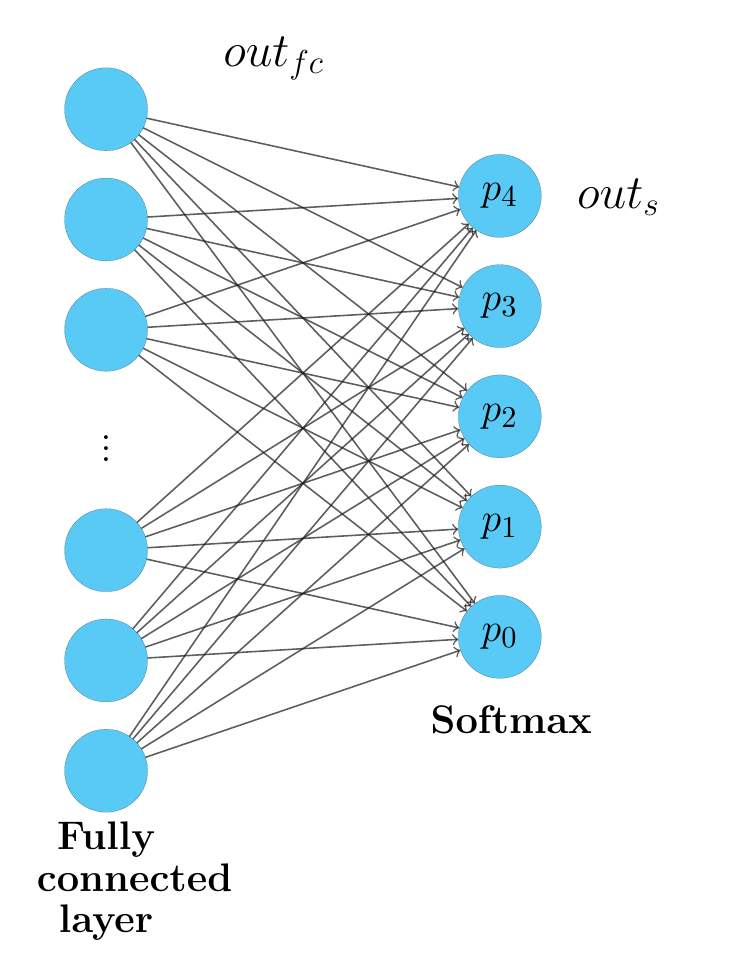
\begin{tikzpicture}
    \fullyConnectedLayer
    
    \softmaxLayer
    
    % Draw connections from fully connected layer to softmax
    \foreach \i in {0,...,\outputnodes} {
        \foreach \j in {1,...,\fcHalfNodes} {
            \draw[connectionNN] (fc-up\j) edge (softmax-\i);
            \draw[connectionNN] (fc-down\j) edge (softmax-\i); 
        }
    }
\end{tikzpicture}

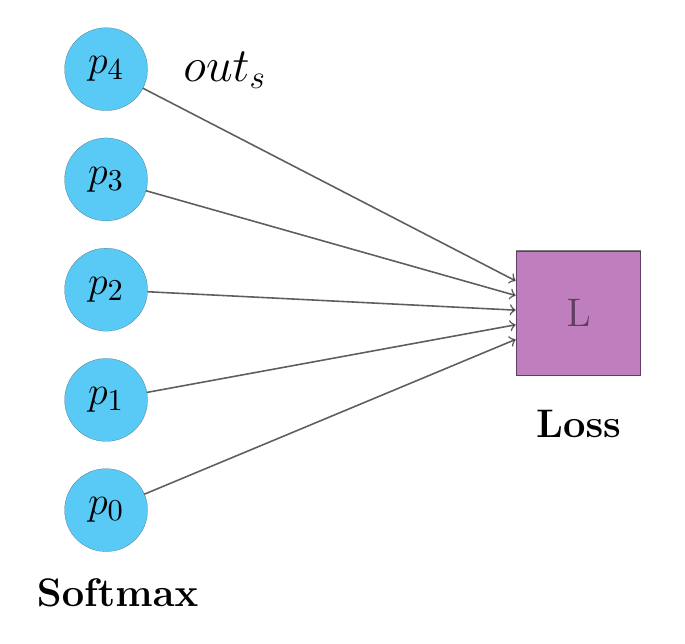
\begin{tikzpicture}
    \softmaxLayer

    \lossLayer

    \foreach \i in {0,...,\outputnodes} {
        \draw[connectionNN] (softmax-\i) edge (L);
    }
\end{tikzpicture}
\end{document}
